\documentclass[a4paper,12pt]{article}

%package Start
\usepackage{graphicx}
\usepackage{titling}
\usepackage{color}
\usepackage{listings}
\usepackage[pdftex,dvipsnames]{xcolor}
\usepackage{nomencl}
\usepackage[graphicx]{realboxes}
\usepackage{rotating}
\definecolor{light-gray}{gray}{0.80}
\usepackage{url}
\usepackage[tight,footnotesize]{subfigure}  
\usepackage[top=2cm, bottom=2cm, left=4cm, right=2cm]{geometry}
\usepackage[colorinlistoftodos,prependcaption,textsize=tiny]{todonotes}
\usepackage{titlesec}
%\usepackage{minted} %for js code


% start of subsubsubsection environment % %
\titleclass{\subsubsubsection}{straight}[\subsection]

\newcounter{subsubsubsection}[subsubsection]
\renewcommand\thesubsubsubsection{\thesubsubsection.\arabic{subsubsubsection}}
\renewcommand\theparagraph{\thesubsubsubsection.\arabic{paragraph}} % optional; useful if paragraphs are to be numbered

\titleformat{\subsubsubsection}
{\normalfont\normalsize\bfseries}{\thesubsubsubsection}{1em}{}
\titlespacing*{\subsubsubsection}
{0pt}{3.25ex plus 1ex minus .2ex}{1.5ex plus .2ex}

\makeatletter
\renewcommand\paragraph{\@startsection{paragraph}{5}{\z@}%
	{3.25ex \@plus1ex \@minus.2ex}%
	{-1em}%
	{\normalfont\normalsize\bfseries}}
\renewcommand\subparagraph{\@startsection{subparagraph}{6}{\parindent}%
	{3.25ex \@plus1ex \@minus .2ex}%
	{-1em}%
	{\normalfont\normalsize\bfseries}}
\def\toclevel@subsubsubsection{4}
\def\toclevel@paragraph{5}
\def\toclevel@paragraph{6}
\def\l@subsubsubsection{\@dottedtocline{4}{7em}{4em}}
\def\l@paragraph{\@dottedtocline{5}{10em}{5em}}
\def\l@subparagraph{\@dottedtocline{6}{14em}{6em}}
\makeatother

\setcounter{secnumdepth}{4}
\setcounter{tocdepth}{4}

% end of subsubsubsection environment % %





\let\abbrev\nomenclature
\renewcommand{\nomname}{List of Abbreviations}
\setlength{\nomlabelwidth}{.25\hsize}
\renewcommand{\nomlabel}[1]{#1 \dotfill}
\setlength{\nomitemsep}{-\parsep}
\makenomenclature 
\newcommand{\Abkuerzung}{
	\printnomenclature
	\newpage
}
%package End

\newcommand{\subtitle}[1]{%
	\posttitle{%
		\par\end{center}
	\begin{center}\large#1\end{center}
	\vskip0.5em}%
}


%\begin{titlepage}
%\begin{center}
\title{XML and NoSQL DBMS: Migration and Benchmarking}
\subtitle{
% TODO->add text from author%
}
%\subtitle{Submitted to the Department of Computer and Information Science at the
%University of Konstanz
%}
%{ \huge \bfseries XML and NOSQL DBMS: Migration and Benchmarking \\[0.4cm] }
%
\includegraphics[width=0.15\textwidth]{./unisignet-klein}~\\[1cm]
\input{includes/first-page/author}
%\end{center}
%\end{titlepage}
\begin{document}
	\definecolor{darkgray}{gray}{0.35}
\lstnewenvironment{fakeXML}[1][]{
\lstset{basicstyle=\footnotesize\sffamily,
linewidth=\linewidth,
breaklines=true, 
%numbers=left,
%stepnumber=1,
%numbersep=10pt,
frame=single,
framerule=1.0pt,
%backgroundcolor=\color{darkgray},
language=HTML,
identifierstyle=\color[rgb]{1,0,0},
emph={intersects}, emphstyle=\color{red},
keywordstyle=\color[rgb]{0,0,1},
commentstyle=\color[rgb]{0.133,0.545,0.133},
stringstyle=\color[rgb]{0.627,0.126,0.941},
morekeywords={xml, ref, xs, version, targetNamespace, minOccurs, maxOccurs}
}\lstset{#1}}{}

\lstnewenvironment{fakeJSON}[1][]{
	\lstset{
		basicstyle=\footnotesize\sffamily,
		keywords={typeof, new, true, false, catch, function, return, null, catch, switch, var, if, in, while, do, else, case, break},
		ndkeywords={class, export, boolean, throw, implements, import, this},
		sensitive=false,
		comment=[l]{//},
		morecomment=[s]{/*}{*/},
		morestring=[b]',
		morestring=[b]"
		linewidth=\linewidth,
		breaklines=true,
		escapeinside={\%*}{*)}
		numbers=left,
		stepnumber=1,
		numbersep=10pt,
		frame=single,
		framerule=1.0pt,
		language=JSON,
		emph={}
	}\lstset{#1}}{}

\colorlet{punct}{red!60!black}
\definecolor{delim}{RGB}{20,105,176}
\colorlet{numb}{magenta!60!black}

\lstdefinelanguage{json}{
	basicstyle=\normalfont\ttfamily,
	linewidth=\linewidth,
	numbers=left,
	numberstyle=\scriptsize,
	stepnumber=1,
	numbersep=8pt,
	showstringspaces=false,
	breaklines=true,
	frame=lines,
	literate=
	*{0}{{{\color{numb}0}}}{1}
	{1}{{{\color{numb}1}}}{1}
	{2}{{{\color{numb}2}}}{1}
	{3}{{{\color{numb}3}}}{1}
	{4}{{{\color{numb}4}}}{1}
	{5}{{{\color{numb}5}}}{1}
	{6}{{{\color{numb}6}}}{1}
	{7}{{{\color{numb}7}}}{1}
	{8}{{{\color{numb}8}}}{1}
	{9}{{{\color{numb}9}}}{1}
	{:}{{{\color{punct}{:}}}}{1}
	{,}{{{\color{punct}{,}}}}{1}
	{\{}{{{\color{delim}{\{}}}}{1}
	{\}}{{{\color{delim}{\}}}}}{1}
	{[}{{{\color{delim}{[}}}}{1}
	{]}{{{\color{delim}{]}}}}{1},
}

	\renewcommand{\lstlistingname}{Code} 
	
	
	\maketitle
	\thispagestyle{empty}
	
	\newpage
	\section*{Abstract}
	XML and NoSQL database are are two growing field in second generation database system, They share some similarities as well as they have some significant difference. 
This thesis focus on the  comparative analysis of these two database system. Based on the Use cases and existing solution, we will discuss the data processing, query pattern and  data retrial from these

	\thispagestyle{empty}	
	\newpage
	\section*{Zusammenfassung(German Abstract)}
	XML und NoSQL
	\newpage
	\section*{Acknowledgments}
	.......................
	\thispagestyle{empty}
	\newpage
	\tableofcontents
	\thispagestyle{empty}
	\newpage
	\section{Introduction}
	\setcounter{page}{1}
	\subsection{Motivation}
		\label{motivation}
			Few years of time XML was  \textit{de facto} data exchange format which enabled people to do previously not that easy thing that time like exchange of content of Microsoft's office documents exchange through HTTP connections. 
	But in recent years a bold transformation has been a foot in the world of Data exchange. The more light weight, less bandwidth consumer JSON(JavaScript Object Notation)[1] has been emerge not just as an alternative to the XML but as rather as potential full Blown successor[2]. Even though these two format has their own pros and cons, the rise of JSON as key in data exchange format, new database technologies so called NoSQL  are also emerges and getting success in their own way. The rate of new research papers in these system are increasing in recent years. 
	
	\subsection{Contribution}
		The main contribution of this thesis is that it provide the necessary techniques and algorithms migration of data from XML database to NoSQL databases.  More specifically, It will focus on Document store databases MongoDB, Couchbase and Rethinkdb. To complete this task it is necessary to understand general architecture and data model of each of these database as well and the Information Retrieval(\textit{IR}).
At the second part, conversion of Queries in XML data to individual NoSQL database is also ......

.....

		
	\subsection{Overview}
		This thesis is divided into three main sections. The first section define the Techniques and necessary algorithms to convert XML  to JSON Data format. The second section will Systems and scope of work. On third section, we see the performance and comparative analysis of each of these systems.
		The work is structured as follows:
		Chapter 2:
		Chapter 3:
		Chapter 4:
		Chapter 5: 
		
	\newpage
	\section{Preliminaries}
		\subsection{Semi-structured data}
		\subsubsection{XML and JSON}
		\subsection{Mapping}
			\subsubsection{Friendly}
			\subsubsection{Unfriendly}
			\subsubsection{Array and Object}
			\subsubsection{Mapping approaches}
			\subsubsection{Summary}
		\subsection{XML Database}
			\subsubsection{XML Query Language}
		\subsection{NoSQL database}
			\subsubsection{Key/Value storage}
			\subsection{document oriented database}
		\subsubsection{Querying NoSQL database}
		
	\newpage
	\section{Related work}
	\newpage
	\section{System/Environment}
		\subsection{BaseX}
			\begin{fakeXML}[label=kml,caption=A simple KML example representing a Point]
<?xml version="1.0" encoding="UTF-8"?>
<kml xmlns="http://www.opengis.net/kml/2.2">
<document>
<placemark>
  <name>New York City</name>
  <description>New York City</description>
  <point>
    <coordinates>-74.006393,40.714172,0</coordinates>
  </point>
</placemark>
</document>
</kml>
\end{fakeXML} 

\begin{fakeJSON}[label=kml,caption=JSON Data]
{"prakash":"Thapa"}
\end{fakeJSON} 


\begin{figure}
	\centering
	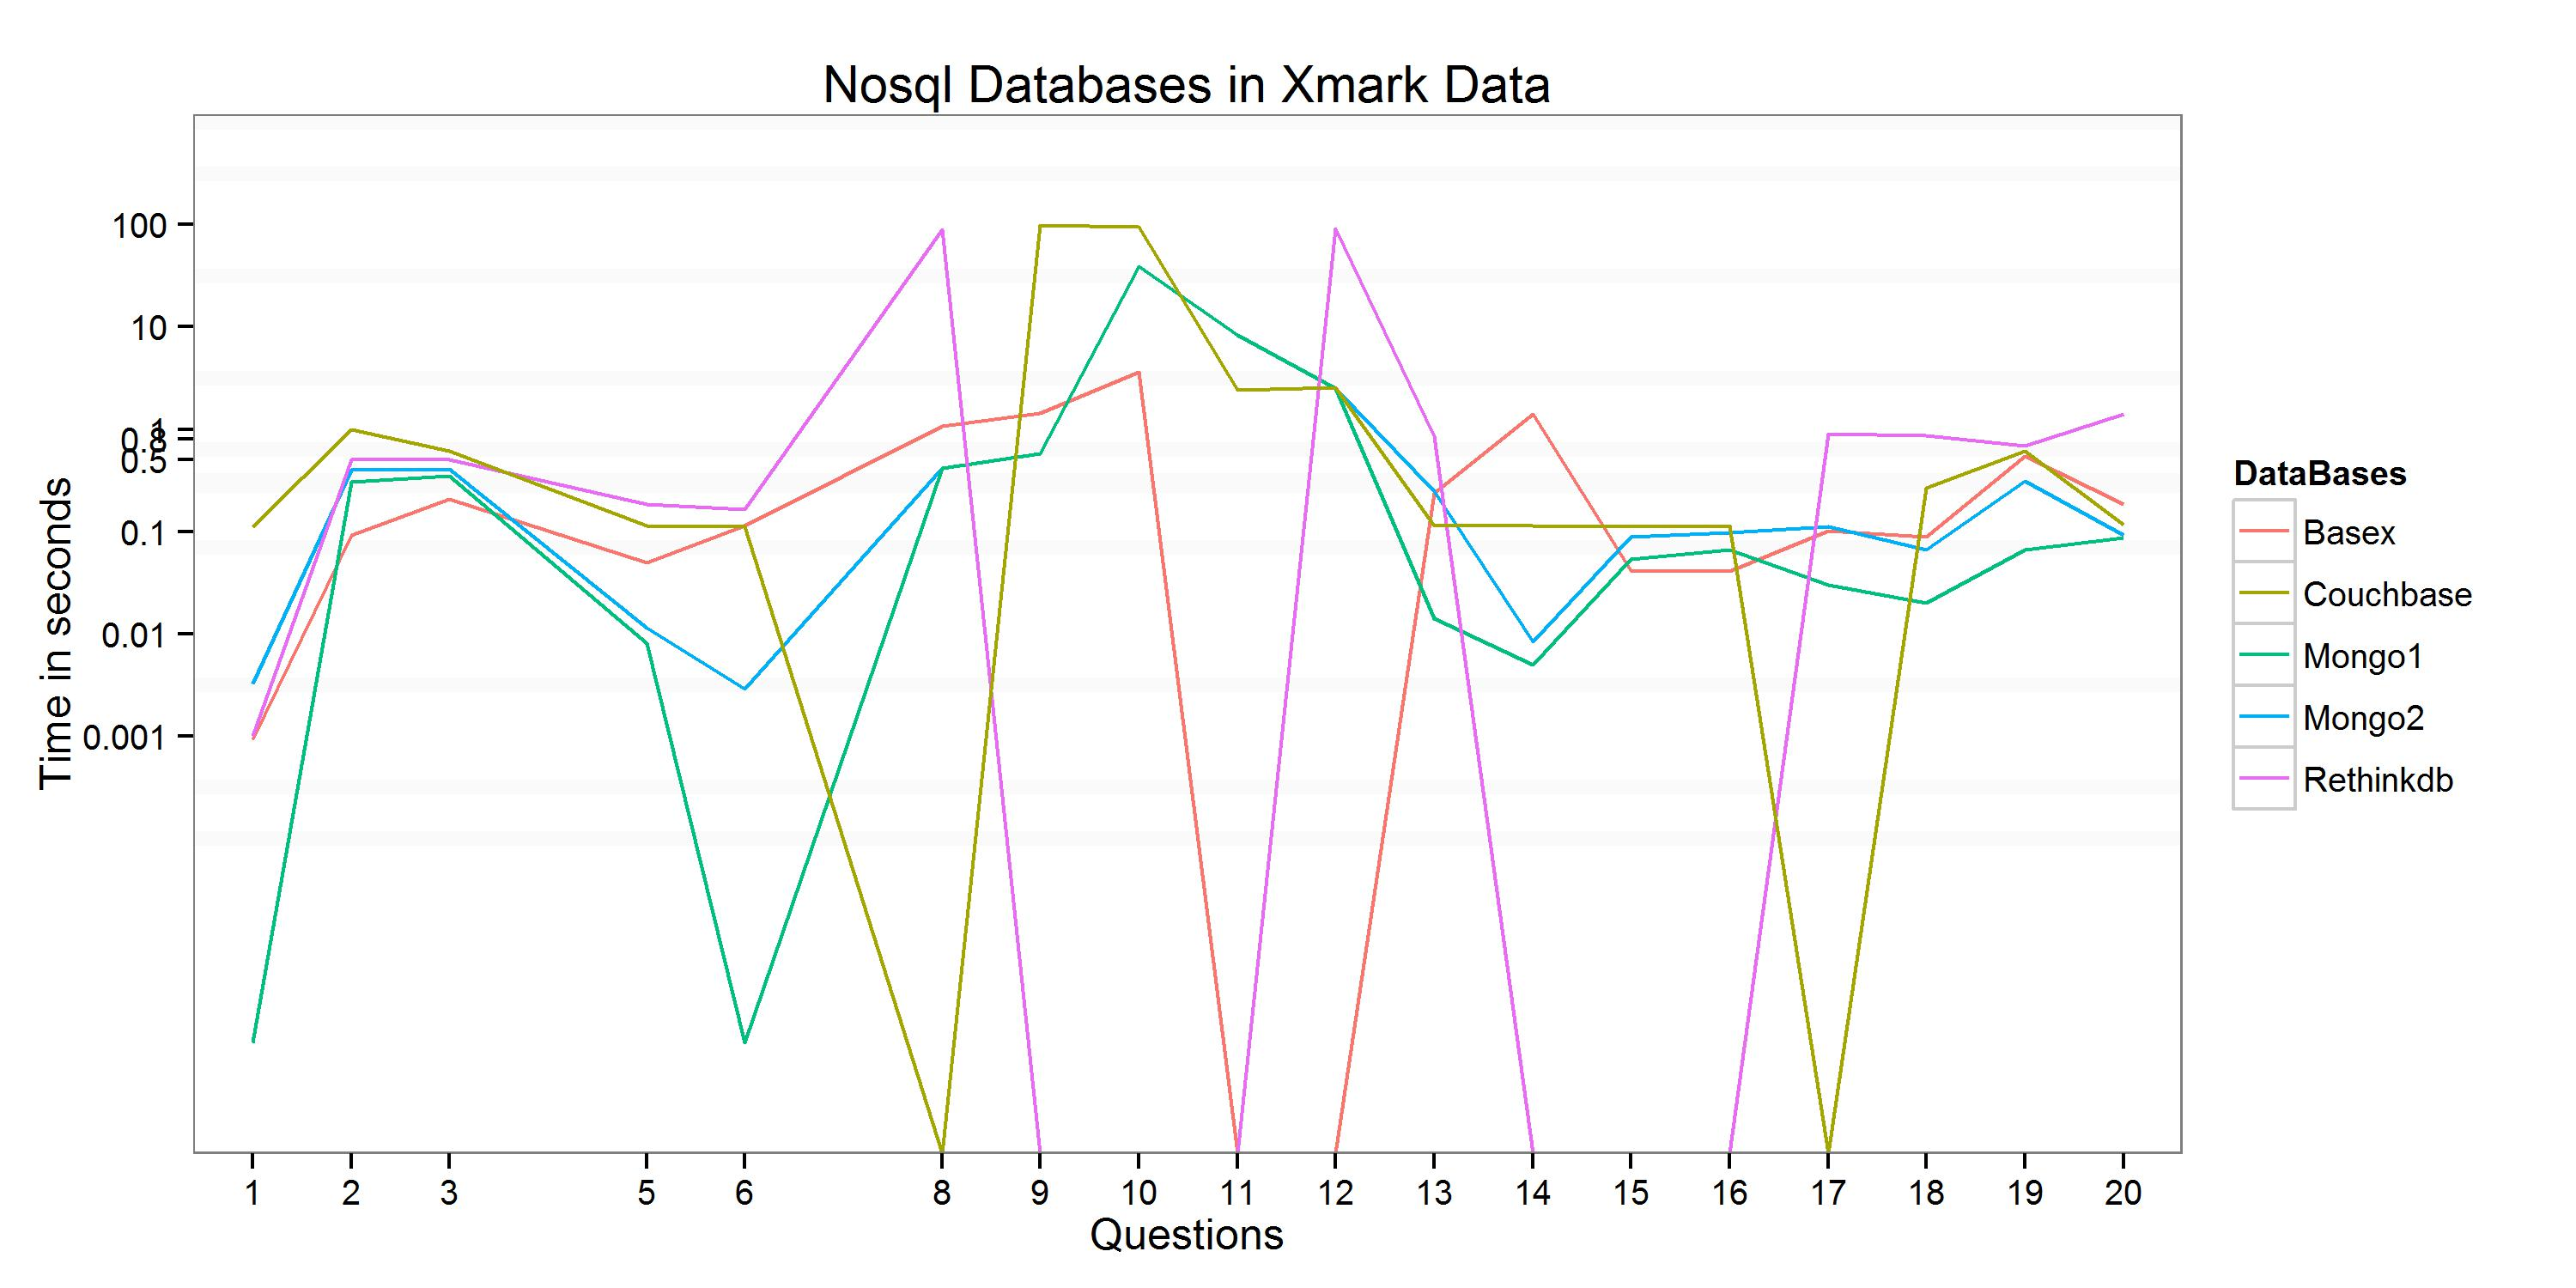
\includegraphics[width=0.9\textwidth]{img/Plot7}
	\caption{An overview of some important indexing structures developed over years}
	\label{trees}
\end{figure}


			
			\newpage
		\subsection{MongoDB}
			%Mongodb is a schemaless document oriented database developed by MongoDB Inc.( then 10gen Inc.) and Open Source Community. It is intended to be flexible data model, fast and Multi-datacenter scalable system written in C++.
\subsubsection{Data Model}
MongoDB uses the concept of \textit{collections} and \textit{documents} to model data. Collection contain any type of documents but generally it has documents with  similar schema. Data has flexible schema where collections do not enforce document to structure rather requirements of our application. A collection is analogous to table of relational database or collection of XML database. Documents are modeled as a data structure following the JSON format which actually store as BSON~\cite{bson}, a binary variant of JSON.  In Mongodb, there are two principle that allow application to represent documents and their relationship: \textit{reference} and \textit{embedded documents}. 
\todo{ need to change following image/json according to xmark data}

\paragraph{Reference}
Reference stores the relationships between data by including links and references from one document to another as in  Figure~\ref{fig:mongodb-ref-doc}. The application can resolve these reference to access the related data\todo{Mongodb data model pg4}
\paragraph{Embedded}
Embedded documents captures relationships between the data by storing related data in a single document structure. The documents in this method are structured as sub-documents\todo{...??} in the in the form of Array or/and Object~\cite{nosql/comparision}. 
\label{mong-xmark-indexing}

\paragraph{Indexing} 
Each document in Mongodb is uniquely identified by a field \textit{\_id} which is a primary index. Hence the collection is sorted by \textit{\_id} by default~\cite{nosql/comparision}.
In addition to primary index, Mongodb supports various user defined indexes for field values of documents including single field index, multikey index, multidimensional index, geo-spatial index, text index and hash index.  Single field, multidimensional and multikey index are organized using B-tree whereas geospatial index is implemented using quad trees.

To index a field that contains a array value, MongoDB provides special indexing called "Multikey". These \textit{multikey} indexes allow MongoDB to return documents from queries using the value of array. 
\begin{figure}
	\centering
	\subfigure[Reference document]{
		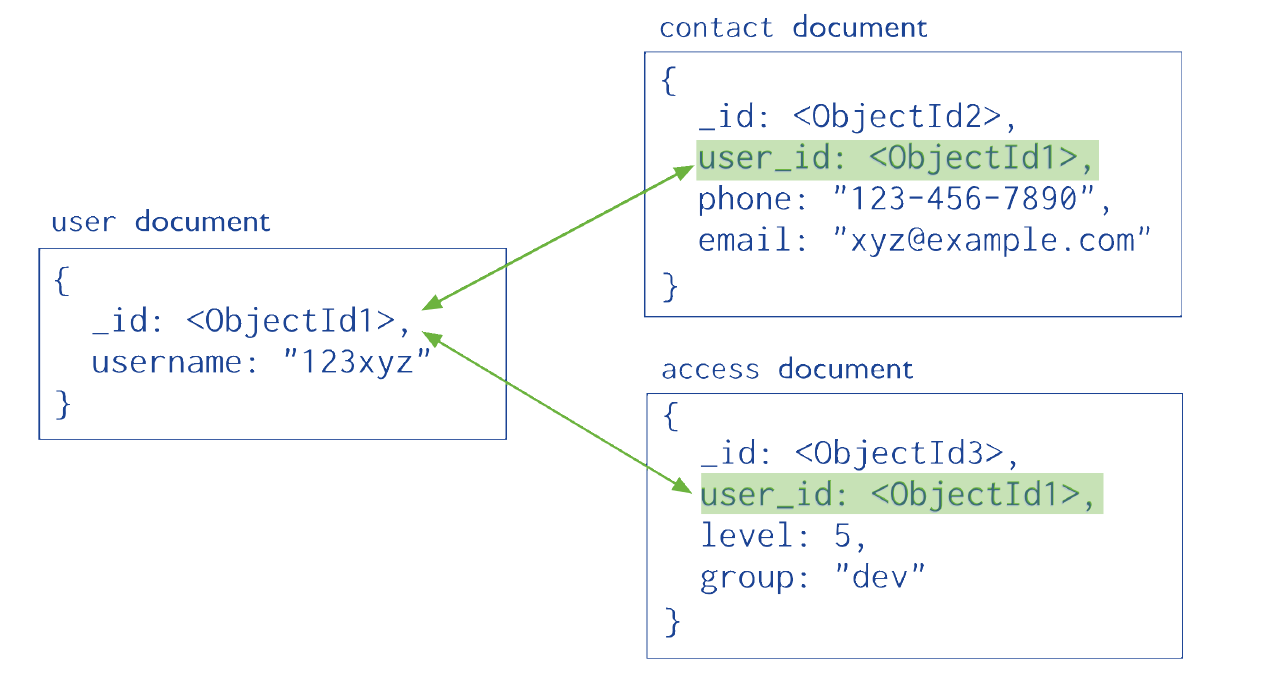
\includegraphics[width=0.44\textwidth]{img/mongodb-reference}
		%\caption{R-tree structure}
		\label{fig:mongodb-ref-doc}
	}
	\centering
	\subfigure[Embedded document]{
		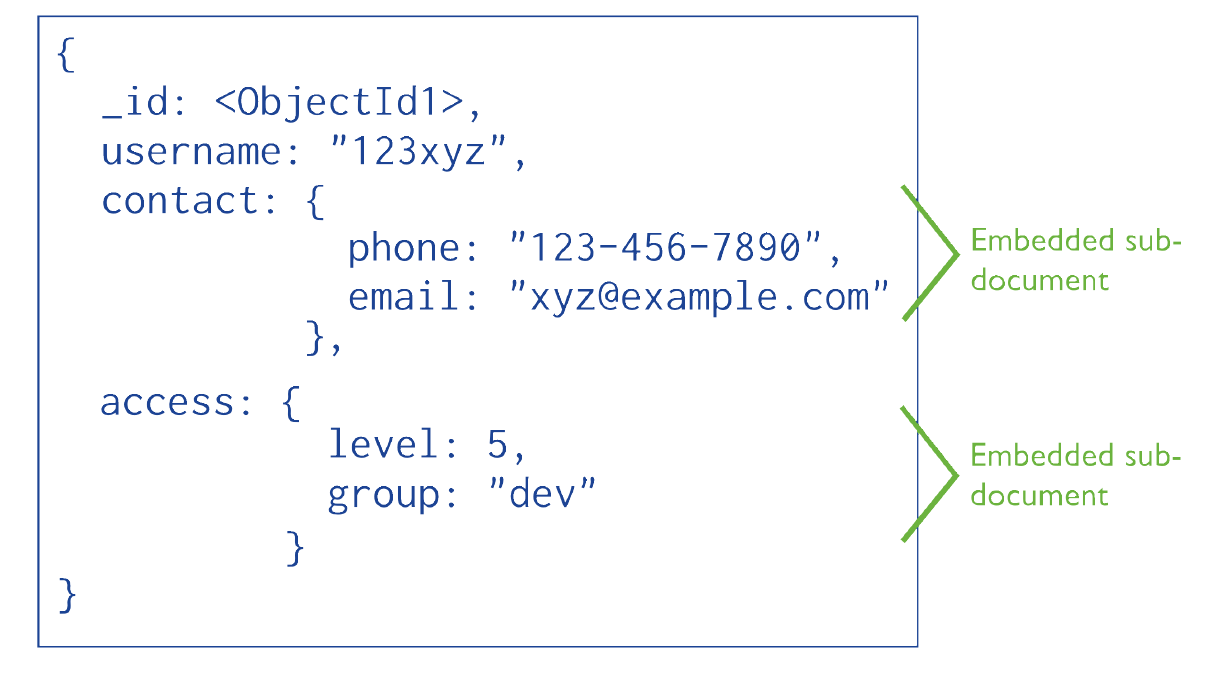
\includegraphics[width=0.44\textwidth]{img/mongodb-embedded}
		%\caption{R-tree}
		\label{fig:mongodb-emb-doc}
	}
	\caption{Mongodb document structure}
	\label{fig:mongodb-doc}
	
\end{figure}

\subsubsection{Query Model}
Queries in MongoDB are expressed in a JSON like syntax and send to MongoDB as BSON objects by database drivers\cite{orend2010analysis}. MongoDB's query can be implemented over all documents inside collections, including embedded object and arrays. 
The Query model support following features:
\begin{enumerate}
	\item Queries over documents, embedded subdocuments and arrays
	\item Comparison operators
	\item Conditional Operators
	\item Logical Operators: AND and OR
	\item Sorting 
	\item Group by 
	\item Aggregation per query
\end{enumerate}
In addition to this MongoDB provide a features to for complex aggregation with the use Of MapReduce. The result of MapReduce either can be store as a collection or be removed after result has been return to client\cite{orend2010analysis}.
		\subsection{Couchbase}
			% Couchbase Server is NoSQL database that can be used both as a key-value store as well as document store system. As key-value store, it is able to store  multiple data type such as strings, numbers, datetime, and booleans as well as arbitrary binary data. The key-value generally treated as opaque Binary Large Object(BLOB) and don't try to parse it. For document store, data need to be store in the valid JSON format.\todo{
  document database system with flexible data model and easily scalable concept~\cite{cb/brown2013developing}}. Data in Couhbase Server are stored in logical unit called Buckets. Buckets are isolated to each other which also have their own RAM quota and replica settings. These buckets can be technically compare as \texttt{database} in Mongodb or other RDBMS. Couchbase recommends as few as possible number of buckets even it is possible to have up to ten bucket in a single cluster system.These buckets can contains theoretically any type of data. All data type other than JSON can be retrieve only by their key. So it is important to check meta type of data stored in a single document before retrieval. 
%In contrast to Mongodb, Couchbase Server don't have concept of collection, documents are separated by the their \texttt{type}.
\paragraph{Metadata}
For every value stored in database, Couchbase Server generate meta information that is associated with the document~\cite{cb/ostrovsky2014pro}. 
	\subparagraph{Expiration}
		The Time to Live(TTL) also named expiration time is the life time of the document. By default it is 0 which indicates it will never expire, also can be set as Unix epoch time after which document is removed. e.g. The maximum number of seconds you can specify are the seconds in a month, namely 2592000(30 x 24 x 60 x 60). Couchbase Server will remove the item after given number of second it stores. 
	\subparagraph{Check-and-Set(CAS)}
		The CAS value is 64-bit integer that is updated by server when associated item is modified and is a method of optimistic locking~\cite{halici1991optimistic}. It enables to update information only if unique identifier matches the identifier of the document that need to be update. CAS is used to manage concurrency when multiple client attempts to update the same document simultaneously. 
	\subparagraph{Flags} 
		Flags are  as 32 bit integer and are set of SDK specific use for SDK specific need. For example, format in which data is serialize or data type of the object being stored. 
	\\ 
	\\
In addition of expiration, CAS and flags, three other meta store at the time of document creation, \texttt{Id}, the document's key is saved as part of metadata. \texttt{type} is the type of document whether it is JSON for all valid JSON documents and \texttt{Base64} for all other than JSON type is being saved as Base64 encoded string.
\paragraph{Document key}
Every value in Couchbase Server has simple or complex \todo{explain simple or complex}  unique key. unlink Mongodb CB don't generate key automatically, it is up to the application creating the data to supply a unique string value up to 250 characters as key for each document~\ref{cb/ostrovsky2014pro}.
%In case of XMark data each \texttt{id} attributes of  \texttt{item}, \texttt{person}, \texttt{open\_auction}, \texttt{category} represent as key. In case of  \texttt{closed\_auction} and  \texttt{edge} key can be manually generated. 
\paragraph{Document design}

\paragraph{Bucket and vBucket}
		\subsection{Rethinkdb}		
			%RethinkDB~\cite{rethindb} is distributed database system to store  JSON documents that uses efficient query languages named ReQL which automatically parallelize queries in multiple machines. ReQL is based on three main principle: it is completely embedded with programming language, ReQL queries can be passed as pipeline from one stage to another to get required result that means it is possible to use series of simple queries together to perform complex operation. Finally, all the queries are executed in server without any intermediate network round trip required the server and clients. 
		\subsection{Summary}
	\newpage
	\section{Performance/Experiments}
		\subsection{XMark}
		\label{xmark}
			The XML benchmarking project XMARK~\cite{xmark/original} dataset is single record with large and complex tree structure. It is one of the most popular and most commonly used XML Benchmark~\cite{xmark/mlynkova2008xml}. It uses a small executable tool called  \textit{xmlgen} that enables to create a synthetic XML Dataset according to fixed DTD of an Internet auction database. The xmlgen produces the dataset that is platform independent and accurately scalable ranging from a minimal document to any arbitrary size limited by the capacity of the system. 
\subsubsection{Dataset}
\label{xmark-dataset}
	XMARK dataset is single record with huge and complicated tree structure ~\cite{xmark/VIST}. 
	%\tikzset{
	basic/.style  = {draw, text width=2cm, drop shadow, font=\sffamily, rectangle},
	root/.style   = {basic, rounded corners=2pt, thin, align=center,
		fill=green!30},
	level 2/.style = {basic, rounded corners=6pt, thin,align=center, fill=green!60,
		text width=8em},
	level 3/.style = {basic, thin, align=left, fill=pink!60, text width=6.5em}
}
\begin{tikzpicture}[
level 1/.style={sibling distance=40mm},
edge from parent/.style={->,draw},
>=latex]

% root of the the initial tree, level 1
\node[root] {Drawing diagrams}
% The first level, as children of the initial tree
child {node[level 2] (c1) {Defining node and arrow styles}}
child {node[level 2] (c2) {Positioning the nodes}}
child {node[level 2] (c3) {Drawing arrows between nodes}};

% The second level, relatively positioned nodes
\begin{scope}[every node/.style={level 3}]
\node [below of = c1, xshift=15pt] (c11) {Setting shape};
\node [below of = c11] (c12) {Choosing color};
\node [below of = c12] (c13) {Adding shading};

\node [below of = c2, xshift=15pt] (c21) {Using a Matrix};
\node [below of = c21] (c22) {Relatively};
\node [below of = c22] (c23) {Absolutely};
\node [below of = c23] (c24) {Using overlays};

\node [below of = c3, xshift=15pt] (c31) {Default arrows};
\node [below of = c31] (c32) {Arrow library};
\node [below of = c32] (c33) {Resizing tips};
\node [below of = c33] (c34) {Shortening};
\node [below of = c34] (c35) {Bending};
\end{scope}

% lines from each level 1 node to every one of its "children"
\foreach \value in {1,2,3}
\draw[->] (c1.195) |- (c1\value.west);

\foreach \value in {1,...,4}
\draw[->] (c2.195) |- (c2\value.west);

\foreach \value in {1,...,5}
\draw[->] (c3.195) |- (c3\value.west);
\end{tikzpicture}
	


\newpage
\begin{figure}
	\centering
	\subfigure[Reference in \textit{XMark} dataset tree Fig~\cite{xmark/original}]{
		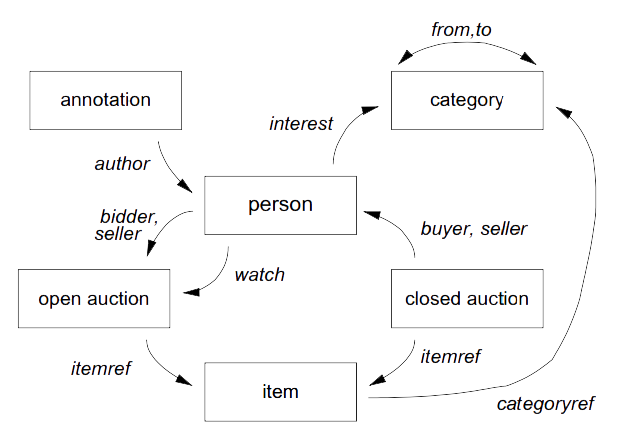
\includegraphics[width=0.40\textwidth]{img/xmark-references.png}{
			\label{xmark-reference}
		}
	}
	\centering
	\subfigure[Reference in \textit{XMark} dataset tree Fig~\cite{xmark/original}]{
		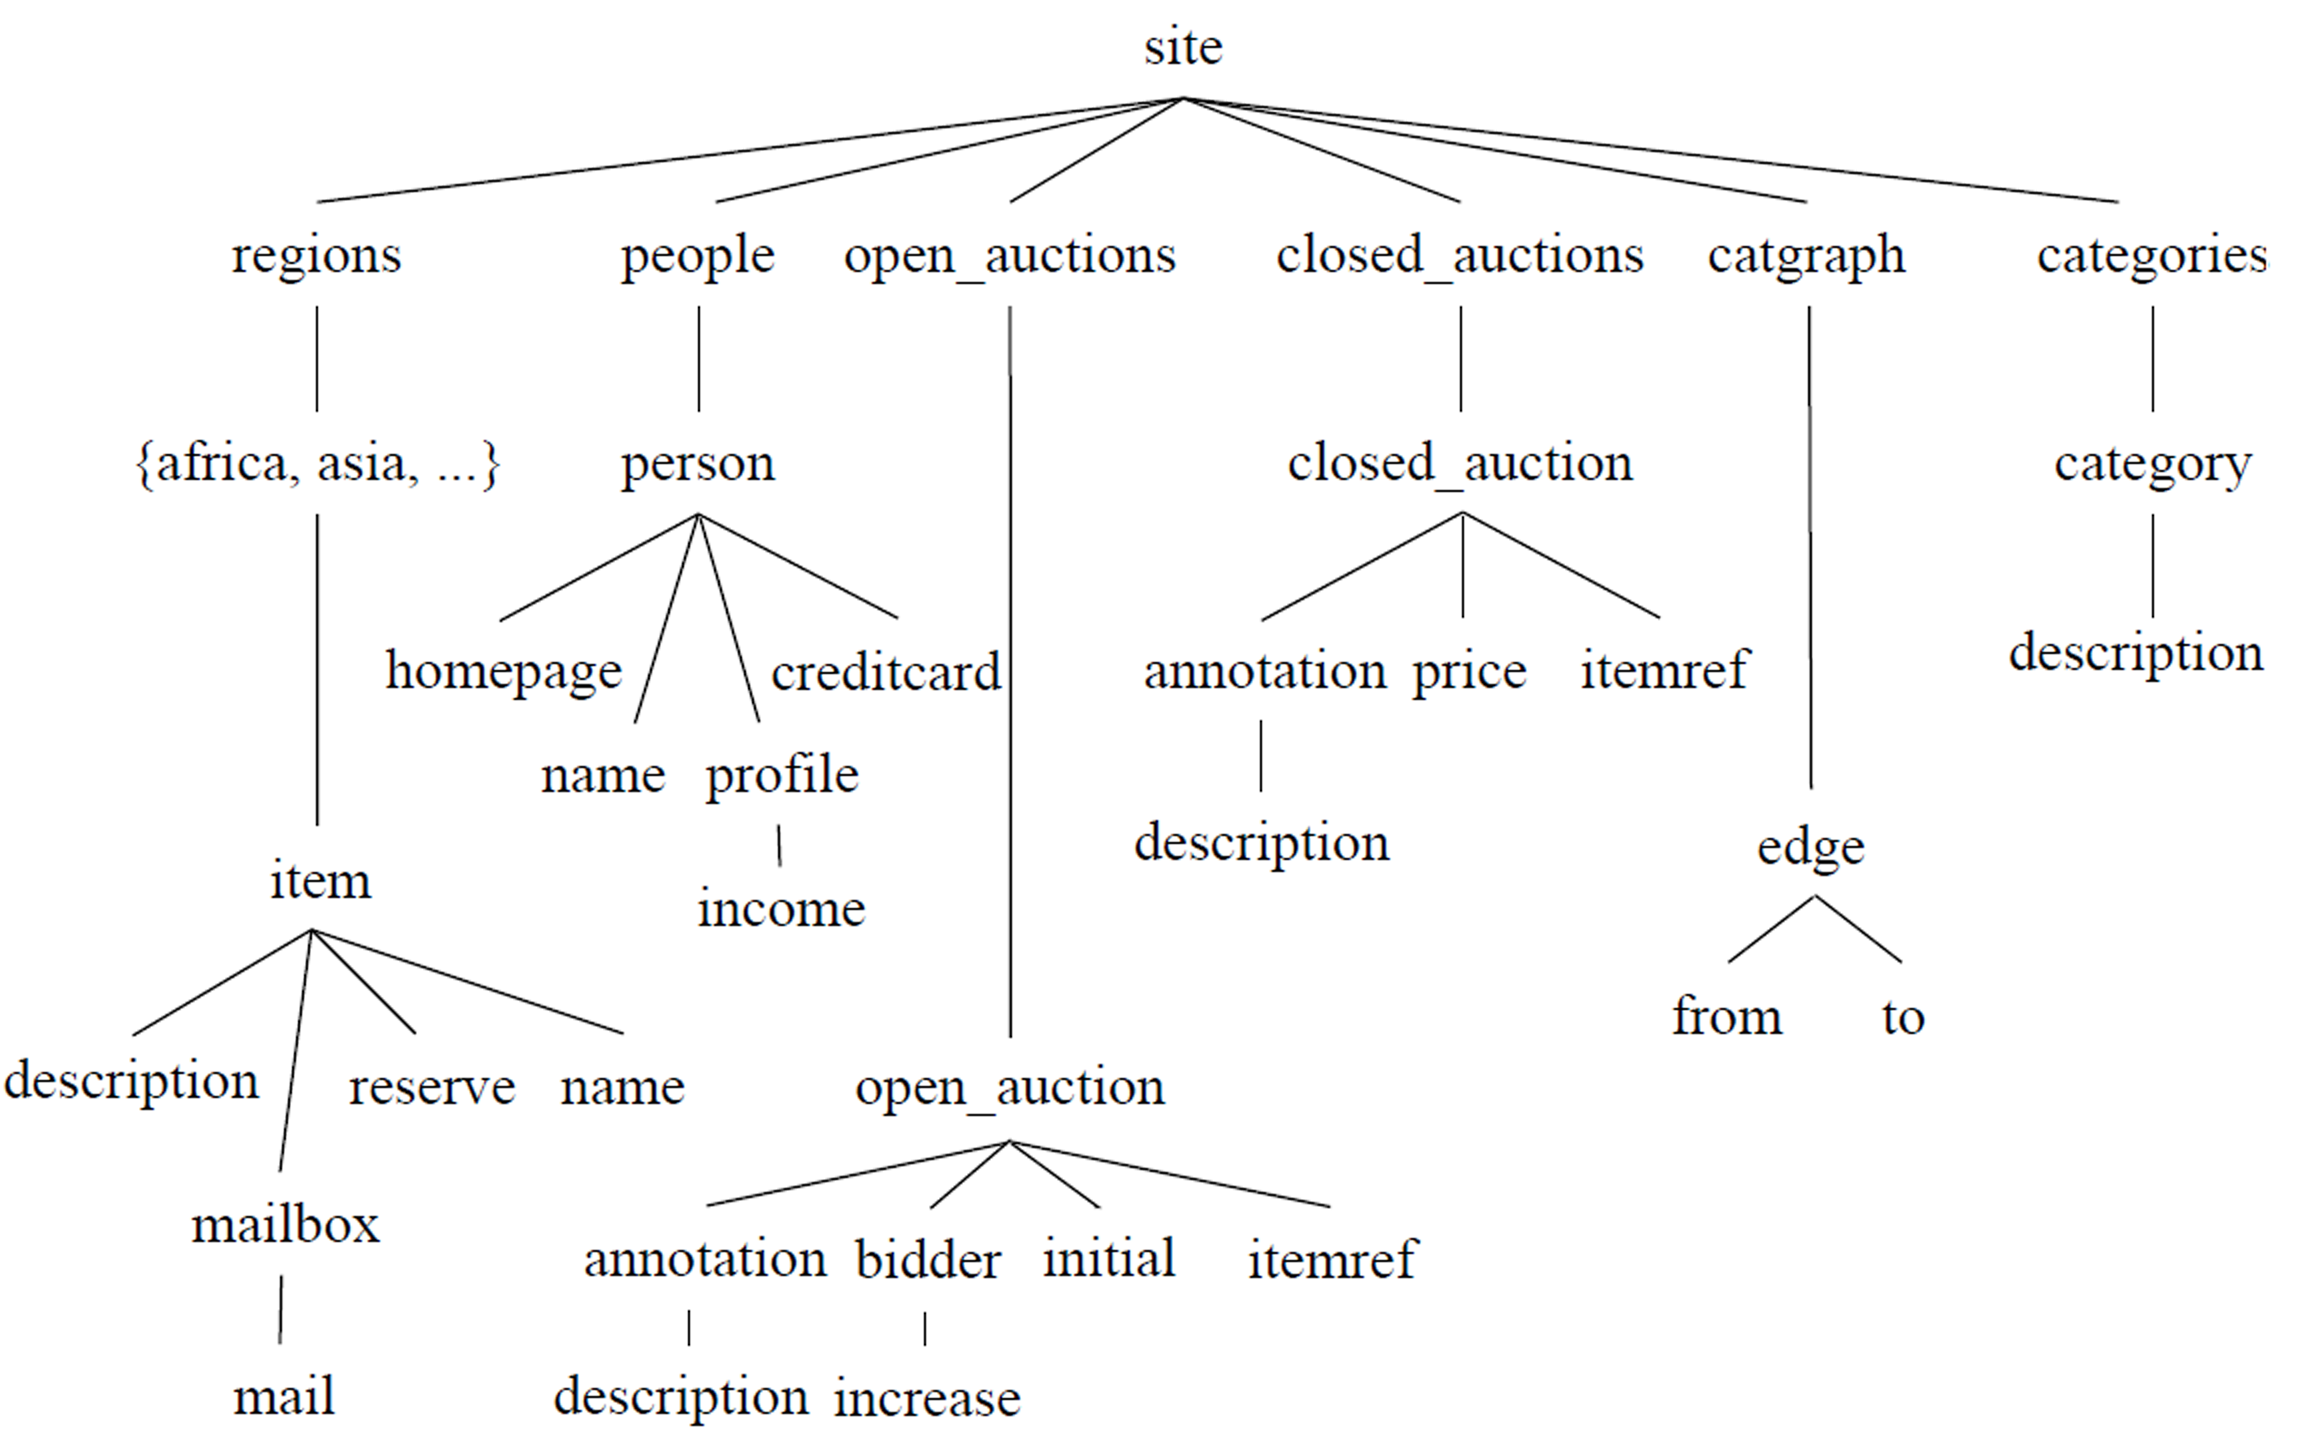
\includegraphics[width=0.40\textwidth]{img/xmark-tree.png}{
			\label{fig:xmark-tree}
		}
	}
	\caption{XMARK data tree and reference}
	\label{fig:xmark-tree-reference}
\end{figure}\todo{figure need to create}

\subsubsection{Queries}
\label{xmark-queries}
coming...
		\subsection{Evaluation of test devices}
		\subsection{XMark data into NoSQL Database}
			A synthetic XMARK dataset consist of one(huge) record in tree structure~\cite{xmark/VIST}. However, As mentioned in \ref{xmark}, each subtree in schema, items, person, open\_auction , closed\_auction etc contains a large number of instances in the database which are indexed in it's own. In most of NoSQL system, this scenario is different, each instance has it's own index structure, the dataset cannot be in just in a huge block rather in decided structure.\todo{This should be elaborated, \textit{language should be imporve}}. As the data modeling of NoSQL do not match this single structure-encoded sequence, we breakdown it's tree structure into set of sub structure without losing the overall data and create index for each of them. As the data modeling from one NoSQL system is different to another unlike most of the XML databases, which have more similar\todo{???} comparison structure than NoSQL. So we need to define modeling for each of those database separately. 			
			\subsubsection{MongoDB}
			\label{xmark-mongodb}
			Data in Mongodb has flexible schema where collections do not enforce document structure rather requirements of our application. There are two principle that allow application to represent documents and their relationship: \textit{reference} and \textit{embedded documents}. 

\todo{ need to change following image according to xmark data}
\begin{figure}
	\centering
	\subfigure[Reference document]{
		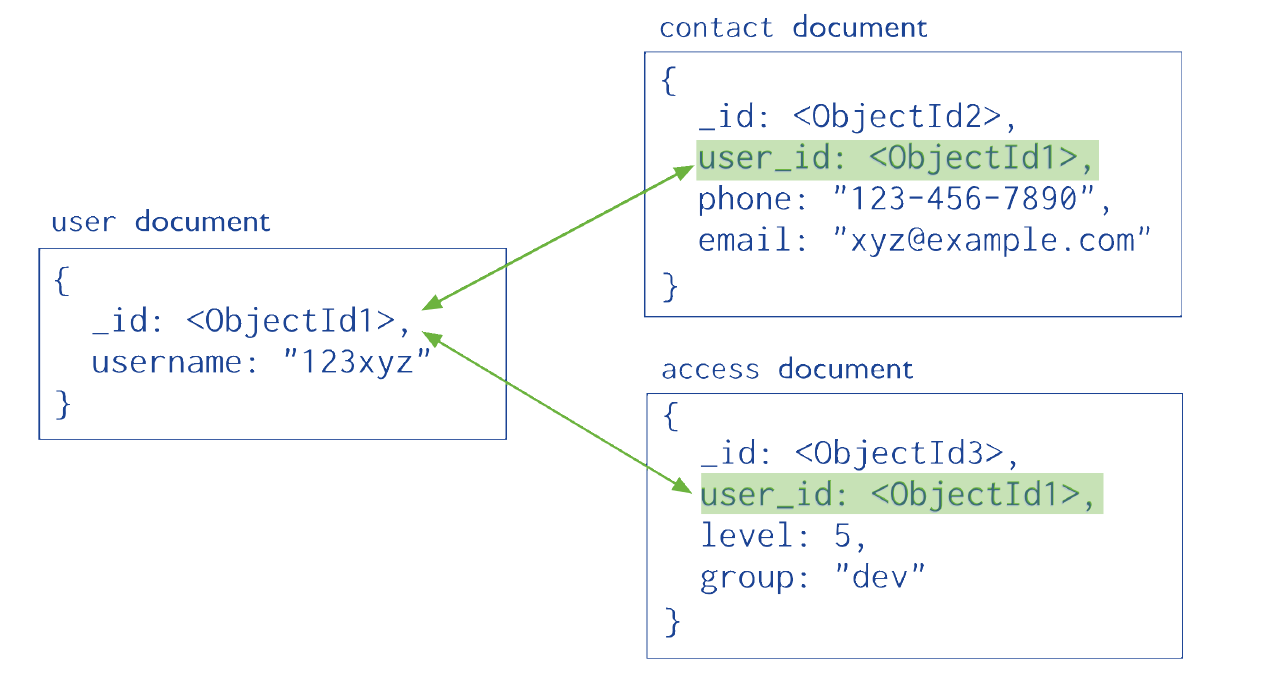
\includegraphics[width=0.44\textwidth]{img/mongodb-reference}
		%\caption{R-tree structure}
		\label{fig:mongodb-ref-doc}
	}
	\centering
	\subfigure[Embedded document]{
		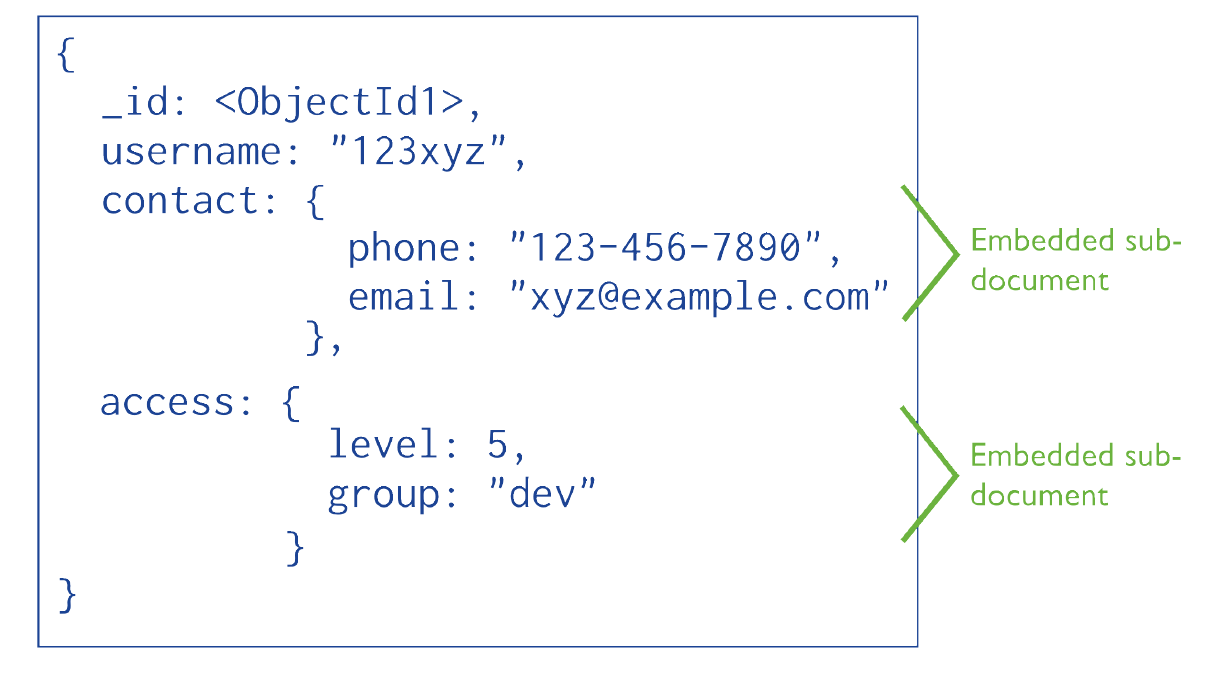
\includegraphics[width=0.44\textwidth]{img/mongodb-embedded}
		%\caption{R-tree}
		\label{fig:mongodb-emb-doc}
	}
	\caption{Mongodb document structure}
	\label{fig:mongodb-doc}
	 
\end{figure}

\paragraph{Reference}
		Reference store the relationships between data by including links and references from one document to another as in  Figure~\ref{fig:mongodb-ref-doc}. The application can resolve these reference to access the related data\todo{Mongodb data model pg4}
\paragraph{Embedded}
	Embedded documents captures relationships between the data by storing related data in a single document structure. The documents in this method are structured as sub-documents\todo{...??} in the in the form of Array or Object. 

			\subsubsection{Couchbase}
			\label{xmark-couchbase}
			\todo{This section has to move to \ref{couchbase-general}}
Couchbase Server is NoSQL document database system with flexible data model and easily scalable concept~\cite{cb/brown2013developing}. Data in Couhbase Server are stored in logical unit called Buckets. Buckets are isolated to each other which also have their own RAM quota and replica settings. These buckets can be technically compare as \texttt{database} in Mongodb or other RDBMS. Couchbase recommends as few as possible number of buckets even it is possible to have up to ten bucket in a single cluster system.These buckets can contains theoretically any type of data(??). All data type other than JSON can be retrieve only by their key. So it is important to check meta type of data stored in a single document before retrieval. 
In contrast to Mongodb, Couchbase Server don't have concept of collection, documents are separated by the their \texttt{doctype}.
\paragraph{Metadata}
For every value stored in database, Couchbase Server generate create metadata that is associated to with the document~\cite{cb/ostrovsky2014pro}. 
	\subparagraph{Expiration}
	\subparagraph{Check-and-Set(CAS)}
	\subparagraph{Flags} 
	\todo{explain in detail}
	\\ 
	\\
In addition of expiration, CAS and flags, three other meta store at the time of document creation, \texttt{Id}, the document's key is saved as part of metadata. \texttt{type} is the type of document whether it is JSON for all valid JSON documents and \texttt{Base64} for all other than JSON type is being saved as Base64 encoded string.
\paragraph{Document key}
Every value in Couchbase Server has simple or complex \todo{explain simple or complex}  unique key. unlink Mongodb CB don't generate key automatically, it is up to the application creating the data to supply a unique string value up to 250 characters as key for each document~\ref{cb/ostrovsky2014pro}.
%In case of XMark data each \texttt{id} attributes of  \texttt{item}, \texttt{person}, \texttt{open\_auction}, \texttt{category} represent as key. In case of  \texttt{closed\_auction} and  \texttt{edge} key can be manually generated. 
\paragraph{Document design}
For Couchbase Server, there is no need to change any structure of XMark NoSQL representation as mentioned in \ref{xmark-nosql} as there is no concept of fragmentation like in \textit{collections} of Mongodb or \textit{tables} in Rethinkdb. The documents are identified by \textit{doctype}. All of these documents are inserted in a single Bucket with \textit{id} as key. For those documents that doesn't have id field, will be manually generated.

\subsubsubsection{Queries}


			\subsubsection{Rethinkdb}
			\label{xmark-rethinkdb}		
		\subsection{Benchmarking}
		\subsection{Summary}
	\newpage
	\section{Discussion}
	\section{Conclusion}
	\label{conc}
	
	\newpage
	\section{Future Work}
	\label{s.future}
	storing in the memory
	\newpage
	\bibliographystyle{unsrt}
	\bibliography{includes/reference}
	\newpage
	\listoffigures
	\newpage
	\listoftables
	\newpage
	\lstlistoflistings
	%%%%%%%%%%%%%%%%%%%%%abkurzen
	\abbrev{dex}{Dalvik Executable}
	\abbrev{XML}{Extensible Markup Language}
	\abbrev{VM}{Virtual Machine}
	\abbrev{JVM}{Java Virtual Machine}
	\abbrev{IPC}{Inter-process Communication}
	\abbrev{SDK}{Software Development Kit}
	\abbrev{GUI}{Graphical User Interface}
	\abbrev{XML}{Extensible Markup Language}
	\abbrev{HTML}{Hypertext Markup Language}
	\abbrev{DOM}{Document Object Model}
	\abbrev{IR}{Information Retrieval}
	
\end{document}	
